\documentclass{article}
\usepackage{hyperref,amsmath,cleveref,graphicx,subcaption}



\title{Location Based Covid-19 Cases Prediction}
\author{Trent Zhang  \\
	Department of Statistics \\
    University of Illinois at Urbana Champaign  \\
	}

\date{\today}
% Hint: \title{what ever}, \author{who care} and \date{when ever} could stand 
% before or after the \begin{document} command 
% BUT the \maketitle command MUST come AFTER the \begin{document} command! 
\begin{document}
\begin{titlepage}
    \begin{center}
        \vspace*{1cm}

        \textbf{Location Based Covid-19 Cases Prediction}

        \vspace{0.5cm}
        Comparison Between Linear Regression and Regression Kriging

        \vspace{1.5cm}

        \textbf{Trent Zhang}
        \vspace{1.5cm}

        \begin{minipage}{30em}
            In this report, we're going to model the spatial structure and the relationship between population and Covid-19 cases in Illinois, Iowa, Wisconsin and Minnesota. As a result, we found the spatial model is better than simple linear regression in performance. The spatial model reached a mean score of 0.48 with cross validation.
        \end{minipage}
        % \begin{figure*}[htp]
        %     \centering
        %     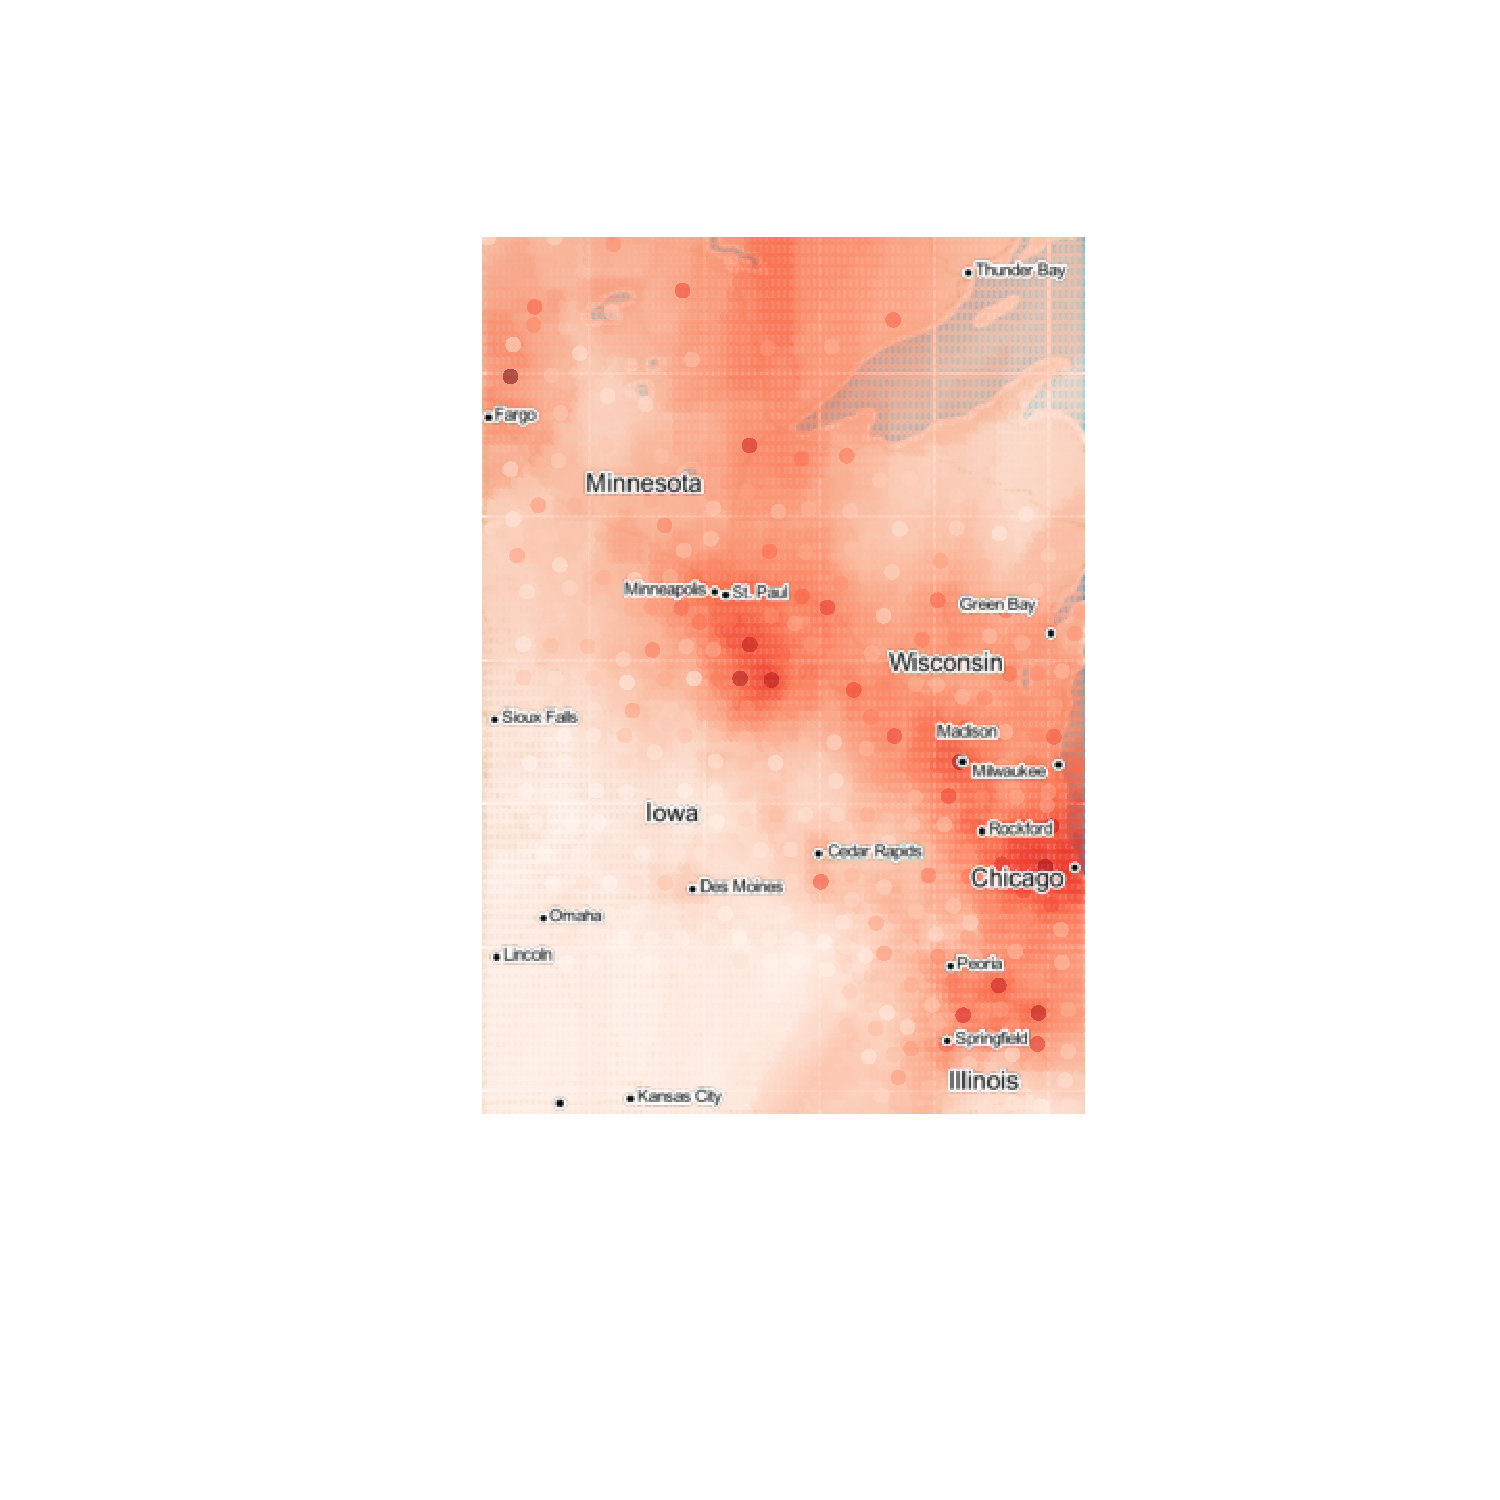
\includegraphics[width=0.3\textwidth]{fig/Cover.pdf}
        % \end{figure*}
        \vfill
        \vspace{0.8cm}

        Department of Statistics\\
        University of Illinois at Urbana-Champaign\\
        United States\\
        \today

    \end{center}
\end{titlepage}


\maketitle


\begin{abstract}
    In this report, we're going to model the spatial structure and the relationship between population and Covid-19 cases in Illinois, Iowa, Wisconsin and Minnesota. As a result, we found the spatial model is better than simple linear regression in performance. The spatial model reached a mean score of 0.48 with cross validation.
\end{abstract}

% The final paper should be about 5/10 pages.
\section{Introduction}
% ∗ Give biological context (1 point)
% ∗ State two scientific questions studied (2 points)
% ∗ Provide rationales for why those two questions are interesting (2 point)
The recent pandemic, which is commonly known as COVID-19, is an infectious disease caused by the virus, severe acute respiratory syndrome coronavirus 2 (SARS-CoV-2). Since the start of the year 2020, the infectious disease COVID-19 has started to spread globally and resulting in almost 517 million positive cases and 6.25 deaths till today.

In this project, we are going to explore the distribution of Covid-19 cases in United States, and will also model the relationship between Covid-19 cases, geographical location and population with Python.

\section{Related Works}
The COVID-19 pandemic is full of unknowns, and many of them have a spatial dimension that lead to understanding the phenomenon as geographical and potentially mappable. Thus from health science, the research needs include the ability to cross variables of different kinds to interpret the COVID-19 phenomenon, its spatial analysis and spatiotemporal dimensions, its geographical impact on decision-making and everyday life, and predictive modelling of the evolution of the disease.

In the paper of Kang et al., the authors explored the spatial epidemic dynamics of COVID-19 in mainland China\cite{kang2020spatial}. Moran's I spatial statistic with various definitions of neighbours was used to conduct a test to determine whether a spatial association of the COVID-19 infections existed. The spatial spread of the COVID-19 pandemic in China was observed. The results showed that most of the models, except medical-care-based connection models, indicated a significant spatial association of COVID-19 infections from around 22 January 2020.

In the paper of Slater et al., they investigated the efficacy of using telecommunication derived mobility data to induce spatial dependence in spatial models applied to two Spanish communities' COVID-19 case counts\cite{slater2021capturing}. They do this by extending Besag York Mollié (BYM) models to include both a physical adjacency effect, alongside a mobility effect. The mobility effect is given a Gaussian Markov random field prior, with the number of trips between regions as edge weights. They leverage modern parametrizations of BYM models to conclude that the number of people moving between regions better explains variation in COVID-19 case counts than physical proximity data. They suggest that this data should be used in conjunction with physical proximity data when developing spatial models for COVID-19 case counts.

From the related works, we can see that the use of geo-spatial and statistical tools has become particularly relevant with the declaration of COVID-19 as a global pandemic.

\section{Data}
% –Materials and methods
% ∗ Describe data source: what it is, where it came from, what technology was used to generate
% the data, briefly how does that technology work (2 points)
\subsection{Data Source}
Our data is collected from CDC\footnote{United States COVID-19 Community Levels by County, \href{https://data.cdc.gov/Public-Health-Surveillance/United-States-COVID-19-Community-Levels-by-County/3nnm-4jnil}{link}}\cite{cdcp}. The \cref{Data Example} shows 2 data example in the original dataset.
\begin{table}[!ht]
    \centering
    \begin{tabular}{lll}
        \hline
        Variable Name                      & Data 1         & Data 2  \\
        \hline
        county                             & American Samoa & Guam    \\
        county fips                        & 60000          & 66000   \\
        state                              & American Samoa & Guam    \\
        county population                  & 47,392         & 168,489 \\
        health service area number         & 901            & 902     \\
        health service area                & American Samoa & Guam    \\
        health service area population     & 47,392         & 168,489 \\
        covid inpatient bed utilization    & 0              & 15.2    \\
        covid hospital admissions per 100k & 2.1            & 38.6    \\
        covid cases per 100k               & 156.14         & 833.88  \\
        covid-19 community level           & Low            & High    \\
        date updated                       & 3/3/22         & 3/3/22  \\
        \hline
    \end{tabular}
    \caption{Data Example}
    \label{Data Example}
\end{table}

From the original data table, we can see that county, county fips, state, county population, health service area number, health service area, covid inpatient bed utilization, covid hospital admissions per 100k, covid cases per 100k, covid-19 community level and date updated are given. In this project, we only use the data in the time period of 2022-04-22 to 2022-05-05, and the attributes of county, state, county population,
% covid hospital admissions per 100k 
and covid cases per 100k for the following analysis. The total data here includes 3224 counties.

\subsection{Data Transformation}
Since the original location data is text based, in order to make numerical analysis, we need to encode the text location into geographical coordinates. Here, we scraped data from Open Street Map to get longitude and latitude of each county in United States\cite{haklay2008openstreetmap}.

Open Street Map is a collaborative project to create a free editable geographic database of the world. The geographical data underlying the maps is considered the primary output of the project. During data scaping, some addresses are failed in search of geographical coordinates, most of them occurred in Puerto Rico and Alaska. In the end, we successfully queried geographical coordinates for 3138 counties, and we only use those data-points to continue analysis.

\subsection{Spatial Data Framework}
We used GeoPandas Data Structures to analysis our data. GeoPandas is an open source project to make working with geospatial data in python easier\cite{jordahl2014geopandas}. GeoPandas extends the datatypes used by pandas to allow spatial operations on geometric types, geometric operations are performed by shapely and Geopandas further depends on fiona for file access and matplotlib for plotting.

\subsection{Preliminary Visualization}
After getting the coordinates data from Open Street Map, we visualized
% covid hospital admissions per 100k 
and covid cases per 100k as in \cref{New Cases Per 100k from 2022-04-22 to 2022-05-05}
% , \cref{New Hospital Admissions Per 100k from 2022-04-22 to 2022-05-05}
. During our visualizations, an abnormal data point in texas was found, we delete that row 35199, and visualize the rest 3137 data points.
\begin{figure}[htbp]
    \centering
    \begin{subfigure}[b]{0.48\textwidth}
        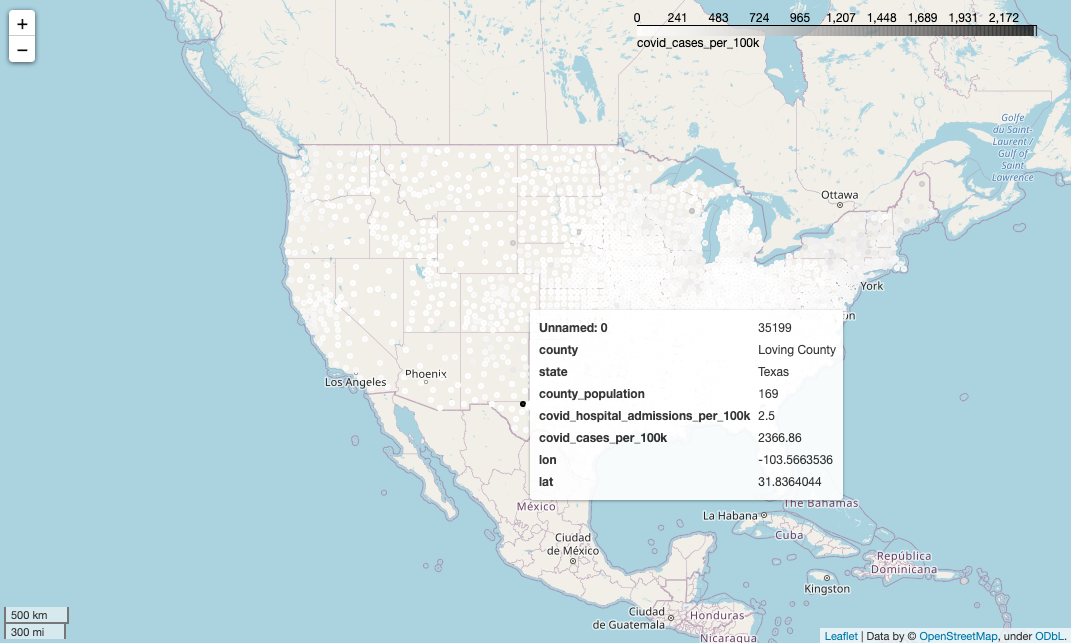
\includegraphics[width=\textwidth]{fig/Suspicious Error Data in Texas.png}
        \caption{Ploy With Abnormal Data}
    \end{subfigure}
    \begin{subfigure}[b]{0.48\textwidth}
        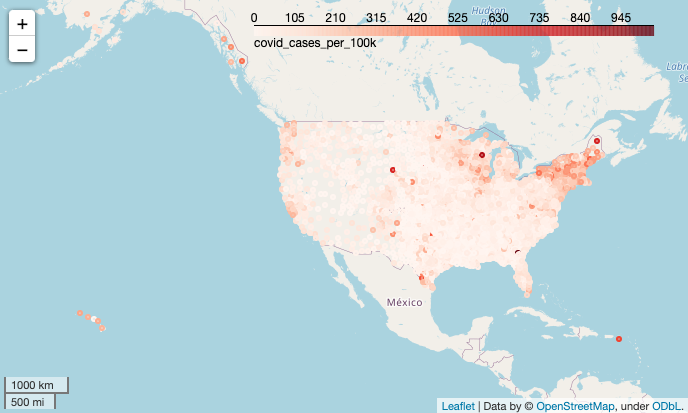
\includegraphics[width=\textwidth]{fig/New Cases from 2022-04-22 to 2022-05-05.png}
        \caption{Plot Without Abnormal Data}
    \end{subfigure}
    \caption{New Cases Per 100k from 2022-04-22 to 2022-05-05}
    \label{New Cases Per 100k from 2022-04-22 to 2022-05-05}
\end{figure}
% \begin{figure}[htbp]
%     \centering
%     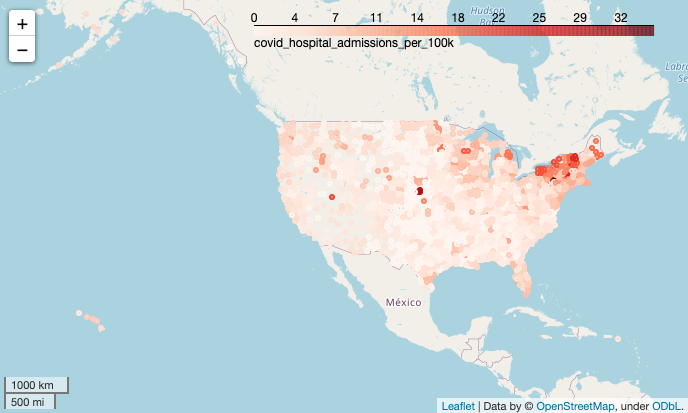
\includegraphics[width=0.8\textwidth]{fig/New Hospital Admissions from 2022-04-22 to 2022-05-05.png}
%     \caption{New Hospital Admissions Per 100k from 2022-04-22 to 2022-05-05}
%     \label{New Hospital Admissions Per 100k from 2022-04-22 to 2022-05-05}
% \end{figure}

\subsection{Vaccination Effect}
As we all agree, vaccination coverage plays a great role in decreasing the Covid-19 cases. Since vaccination can greatly affect Covid-19 cases and vaccination coverages are significantly different between different states. Therefore, the model will be unreliable if we didn't consider vaccination rate as a influential factor.

However, The vaccination data at CDC are missing in many counties, thus requiring more time to clean the data. Due to the time limitation, we don't consider vaccination as an influential factor here.

In order to make vaccination effect ignorable, we only analyze the data in Illinois, Iowa, Wisconsin and Minnesota, which have similar vaccination coverage according to \cref{Vaccination Coverage} from CDC
\footnote{From Centers for Disease Control and Prevention, \href{https://covid.cdc.gov/covid-data-tracker}{link}}. The final data points visualization is as \cref{Final Data Points}.

\begin{figure}[htbp]
    \centering
    \begin{minipage}{0.7\textwidth}
        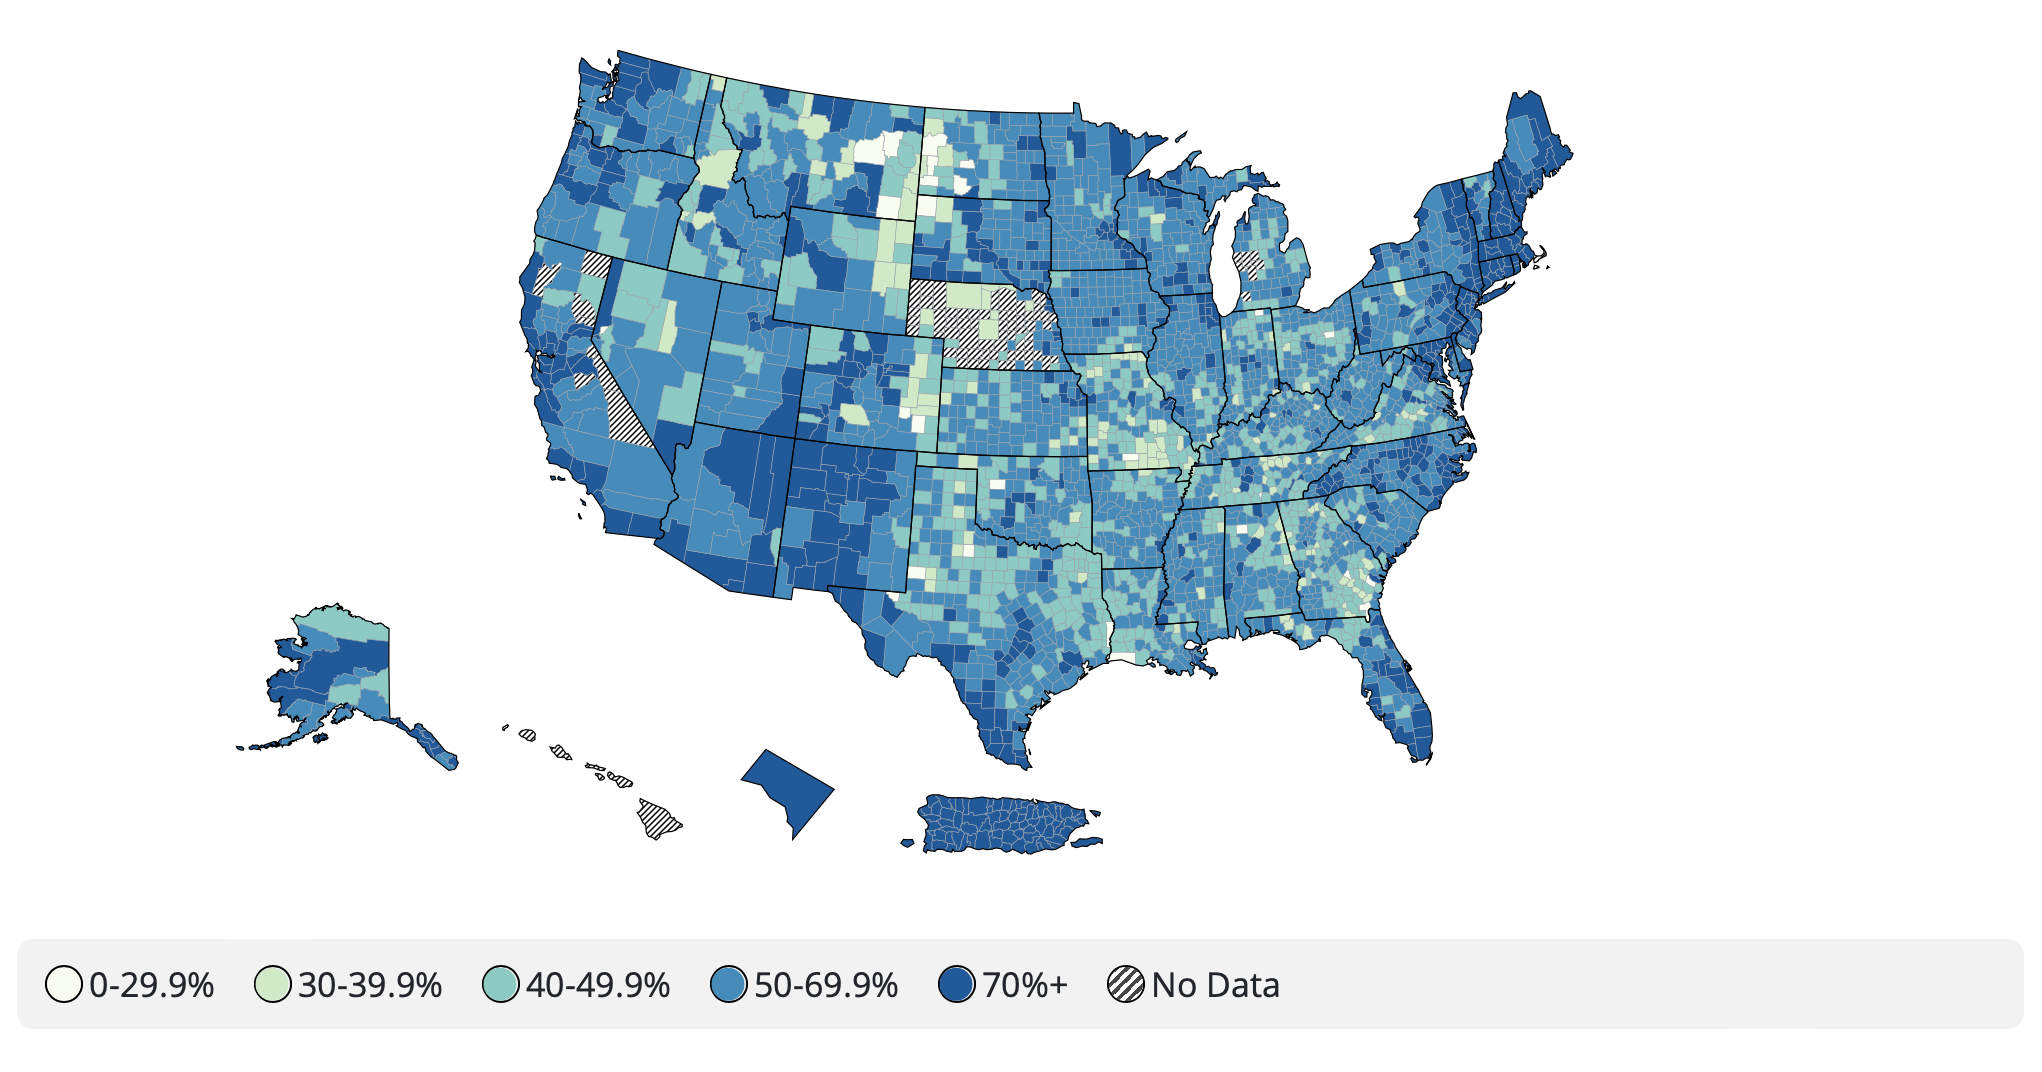
\includegraphics[width=\textwidth]{fig/Vaccination Plot.png}
        \caption{Vaccination Coverage}
        \label{Vaccination Coverage}
    \end{minipage}\hfill
    \begin{minipage}{0.3\textwidth}
        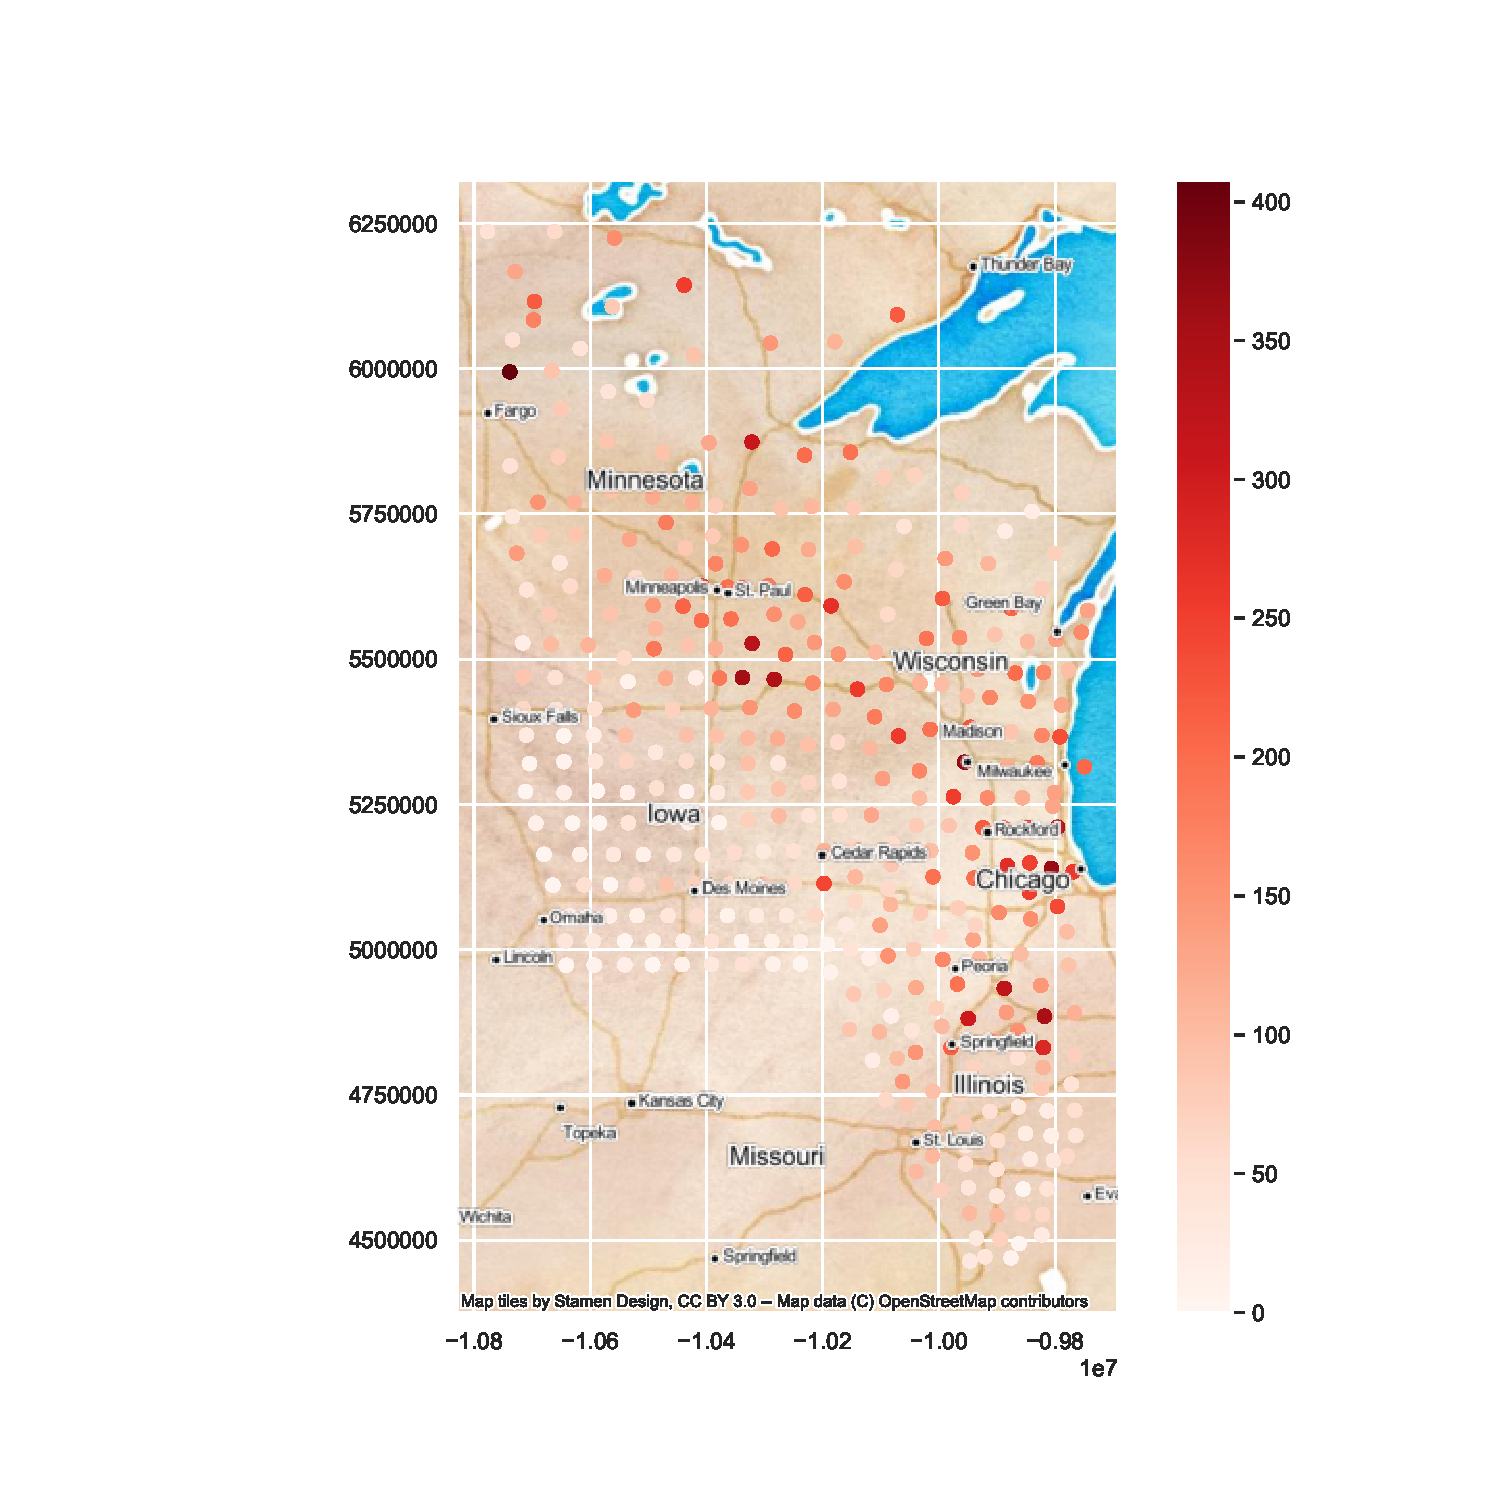
\includegraphics[width=\textwidth]{fig/Data Points.pdf}
        \caption{Data Points}
        \label{Final Data Points}
    \end{minipage}
\end{figure}
% \begin{figure}[htbp]
%     \centering
%     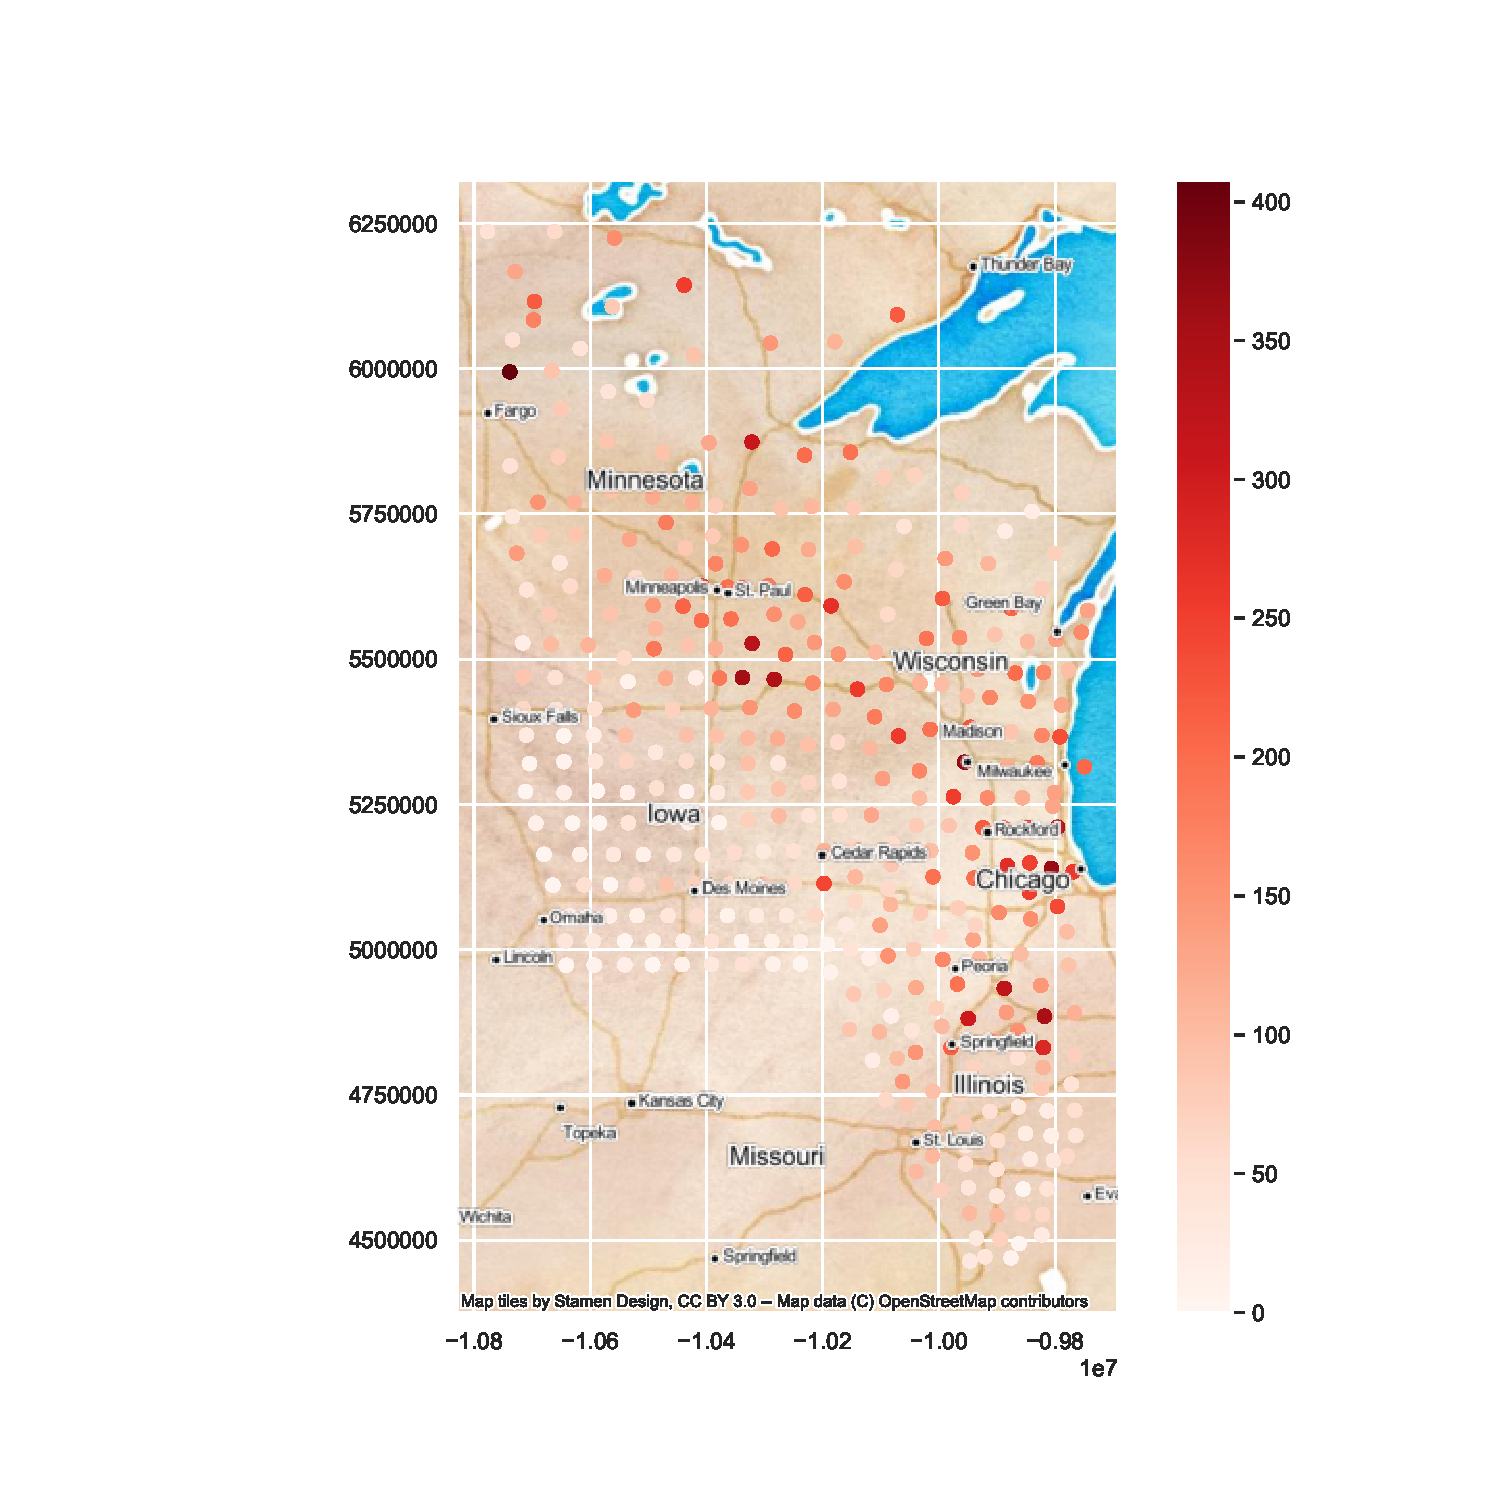
\includegraphics[width=0.7\textwidth]{fig/Data Points.pdf}
%     \caption{Final Data Points}
%     \label{Final Data Points}
% \end{figure}

\section{Methods}
% ∗ Describe statistical methods used to analyze the data (2 points)
% ∗ Report software and packages used for the analysis (1 point)

\subsection{Simple Linear Regression}


% \subsubsection{Relationship Visualization}
\begin{figure}[htbp]
    \centering
    \begin{subfigure}[b]{0.48\textwidth}
    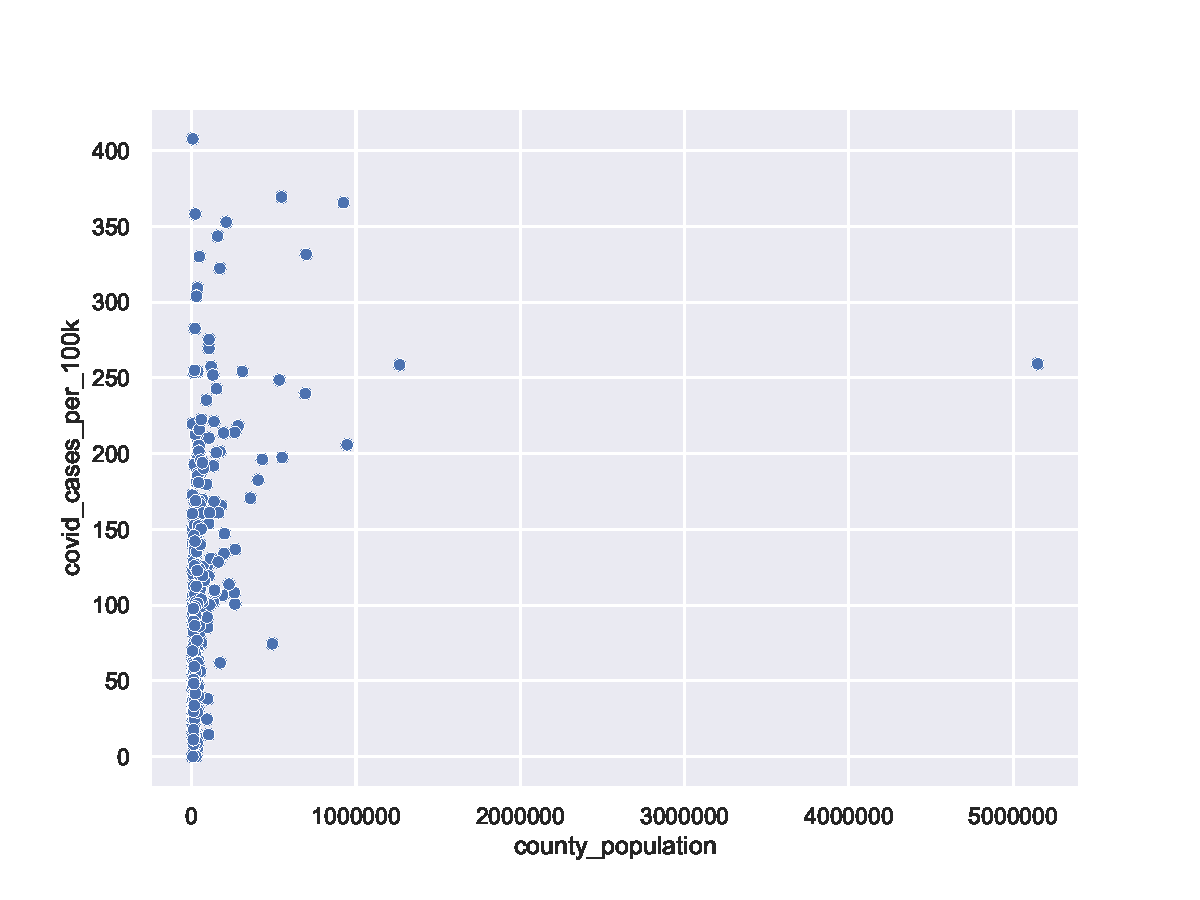
\includegraphics[width=\textwidth]{fig/Relationship Between Population and Cases.pdf}
    \caption{Without Logarithm}
\end{subfigure}
\begin{subfigure}[b]{0.48\textwidth}
    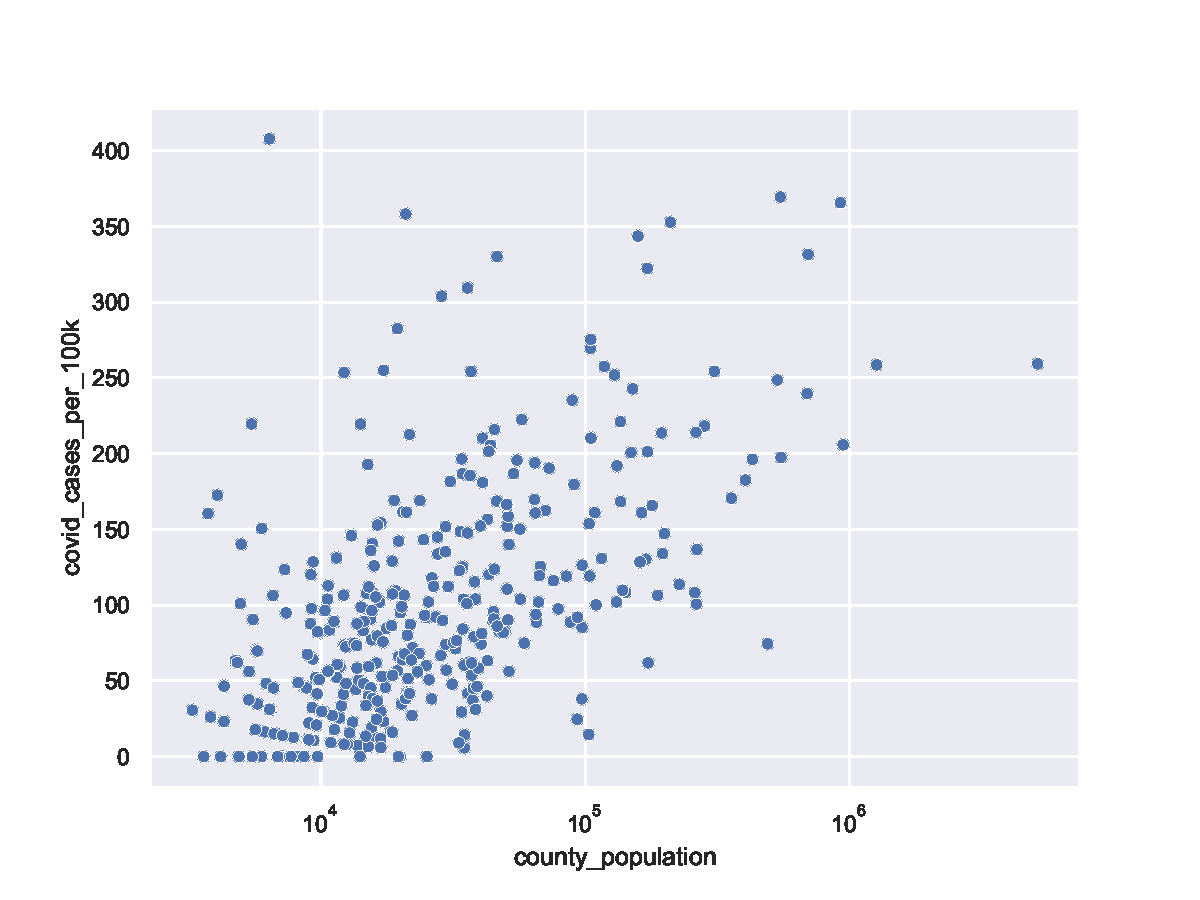
\includegraphics[width=\textwidth]{fig/Relationship Between Population and Cases (Log).pdf}
    \caption{With Logarithm}
\end{subfigure}
    \caption{Relationship Visualizations}
    \label{Relationship Visualizations}
\end{figure}

In \cref{New Cases Per 100k from 2022-04-22 to 2022-05-05}, we first visualized the relationship between county population and covid cases per 100k, however, there seems no linear relationship between them. Then we  visualized the relationship between log county population and covid cases per 100k, then we can notice increasing trend in our plot. Therefore, we use the log county population as our variable.

Besides, we also normalized all the data before linear regress our model, therefore, there will be no intercept term in our model. The simple linear regression model is as:
\begin{equation}
    y=x\beta+\epsilon
\end{equation}
where:
\begin{itemize}
    \item $y$: covid cases per 100k
    \item $x$: log county population
    \item $\beta$: coefficient of log county population
    \item $\epsilon$: random gaussian noise
\end{itemize}

Here we used Scikit-learn Framework in python to implement simple linear regression\cite{pedregosa2011scikit}.  Scikit-learn (formerly scikits.learn and also known as sklearn) is a free software machine learning library for the Python programming language. It features various classification, regression and clustering algorithms including support-vector machines, random forests, gradient boosting, k-means and DBSCAN, and is designed to interoperate with the Python numerical and scientific libraries NumPy and SciPy.
\subsection{Regression Kriging}
The simple linear regression didn't capture the spatial dependence between different counties. In this section, we are going to talk about Regression Kriging which can model the spatial dependence between locations.

Here we used GeoStatTools in GeoStat Framework in python to implement regression kriging\cite{muller2022gstools}.  GeoStatTools is a library providing geo-statistical tools like kriging, random field generation, variogram estimation and user-defined covariance models.

\subsubsection{Model Form}
Regression kriging is an implementation of the best linear unbiased predictor (BLUP) for spatial data, i.e. the best linear interpolator assuming the universal model of spatial variation. This model proposed that a value of a target variable at some location can be modeled as a sum of the deterministic and stochastic components:
\begin{equation}
    y( s )=m( s )+\varepsilon^{\prime}( s )+\varepsilon^{\prime \prime}
\end{equation}
\begin{itemize}
    \item ${y}\left( s\right)$ is the target value at location $s$;
    \item ${m}\left( s\right)$ is the fitted deterministic part;
    \item $\varepsilon^{\prime}( s )$ is the interpolated residual at location $s$;
    \item $\varepsilon^{\prime \prime} $ is the remaining residual.
\end{itemize}
In our case, the deterministic part is $x( s )\beta$, by combining the two approaches, we obtain:
\begin{equation}
    y( s )=x( s )\beta+\varepsilon^{\prime}( s )+\varepsilon^{\prime \prime}
\end{equation}

In order to estimate the interpolated residual at location $s$, which is $\varepsilon^{\prime}( s )$, we introduce Kriging here.
Kriging predicts the value of a function at a given point by computing a weighted average of the known values of the function in the neighborhood of the point. Depending on the stochastic properties of the random field and the various degrees of stationarity assumed, different methods for calculating the weights can be deduced, i.e. different types of
kriging apply. There are 2 classical methods:
\begin{enumerate}
    \item Ordinary kriging assumes constant unknown mean only over the search neighborhood of $s_{0}$.
          % \item Simple kriging assumes stationarity of the first moment over the entire domain with a known mean: $E\{y(s)\}=E\left\{y\left(s_{0}\right)\right\}=m$, where $m$ is the known mean.
    \item Universal kriging assumes a general polynomial trend model, such as linear trend model $E\{y(s)\}=\sum_{k=0}^{p} \beta_{k} f_{k}(s)$.
\end{enumerate}

\subsubsection{Variogram models}
The theoretical variogram $2 \gamma\left( s _{1}, s _{2}\right)$ is a function describing the degree of spatial dependence of a spatial random field or stochastic process $y( s )$. The semivariogram $\gamma\left( s _{1}, s _{2}\right)$ is half the variogram.

In the our case, a variogram will give a measure of how much two samples taken from the area will vary in Covid cases depending on the distance between those samples. Samples taken far apart will vary more than samples taken close to each other.

In this project, we consider the following 4 variogram models:
\begin{enumerate}
    \item Linear $$
        \rho(s)= \begin{cases}1-\sigma \cdot \frac{s}{\ell} & s<\frac{\ell}{\sigma} \\ 0 & s \geq \frac{\ell}{\sigma}\end{cases}
        $$
    \item Power $$
        \gamma(s)=\sigma^{2}\left(1-\exp \left(-\sigma \cdot \frac{s}{\ell}\right)\right)+n
        $$
    \item Gaussian $$\gamma(s)=\sigma^{2}\left(1-\exp \left(-\left(\sigma \cdot \frac{s}{\ell}\right)^{2}\right)\right)+n$$
    \item Spherical $$\rho(s)= \begin{cases}1-\frac{3}{2} \cdot \sigma \cdot \frac{s}{\ell}+\frac{1}{2} \cdot\left(\sigma \cdot \frac{s}{\ell}\right)^{3} & s<\frac{\ell}{\sigma} \\ 0 & s \geq \frac{\ell}{\sigma}\end{cases}$$
\end{enumerate}




\section{Results and Discussion}
% ∗ Perform at least 5 analyses and report the results; your report should contain numbers/p-values/etc (5 points)
% ∗ Provide at least 2 visualizations (2 points)
\subsection{Best Model}
In order to evaluate the prediction accuracy, we use coefficient of determination to evaluate our models, and we use 10 fold cross validation for model selection, the result is as \cref{Regression vs Kriging}, \cref{Regression Kriging}. 

From \cref{Regression vs Kriging}, we can see that Simple regression has low score around 0.1, however, the regression kriging model has a much higher score around 0.5. This means that there are indeed spatial dependence structure in our data, and it can greatly improve the accuracy of prediction. 

From \cref{Regression vs Kriging}, we can see that among all variograms and kriging methods we tried, the Ordinary Kriging with Spherical variogram works the best, with mean score of 0.48. 

\begin{figure}[htbp]
    \centering
    \begin{minipage}{0.5\textwidth}
        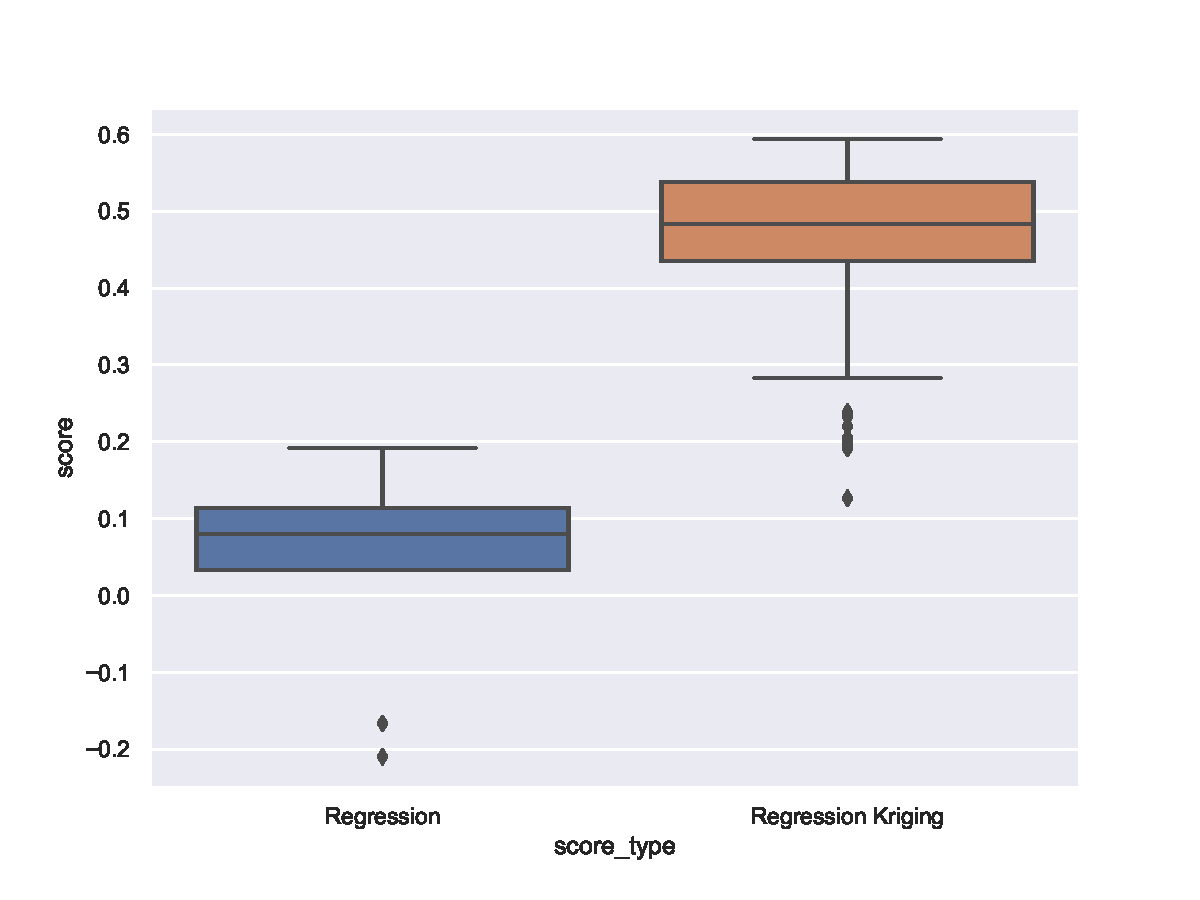
\includegraphics[width=\textwidth]{fig/Regression vs Regression Kriging.pdf}
        \caption{Simple vs Kriging}
        \label{Regression vs Kriging}
    \end{minipage}\hfill
    \begin{minipage}{0.5\textwidth}
        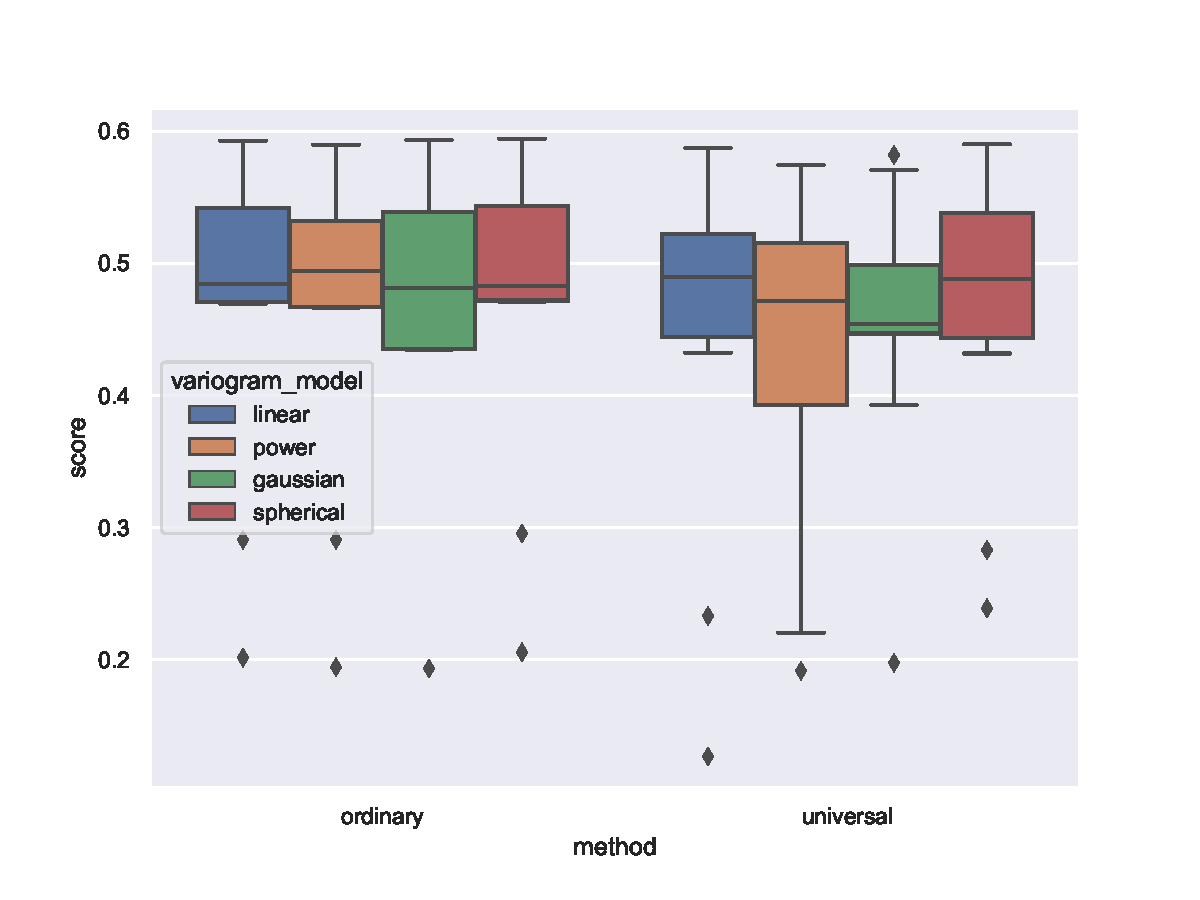
\includegraphics[width=\textwidth]{fig/Regression Kriging.pdf}
        \caption{Regression Kriging}
        \label{Regression Kriging}
    \end{minipage}
\end{figure}

\subsection{Prediction}
Here, we will show the prediction result in Illinois, Iowa, Wisconsin and Minnesota areas. First, we need to create a prediction grid in this area, a uniformly distributed grid of 100 by 100 is created as in \cref{Prediction Grid}.

After the grid is created, for each point on grid, we use the population its closest county as its population. Then we use our selected model to predict on the grid data points. The predicted result is as \cref{Prediction}, the background red color is the predicted value on the grid, and the red dot is the actual value from our training data. 

From the plot, we can see that the dots in the places which have peak Covid-19 cases are more observable than others, which means that our model is bad at predicting extreme values. 
\begin{figure}[htbp]
    \centering
    \begin{minipage}{0.62\textwidth}
        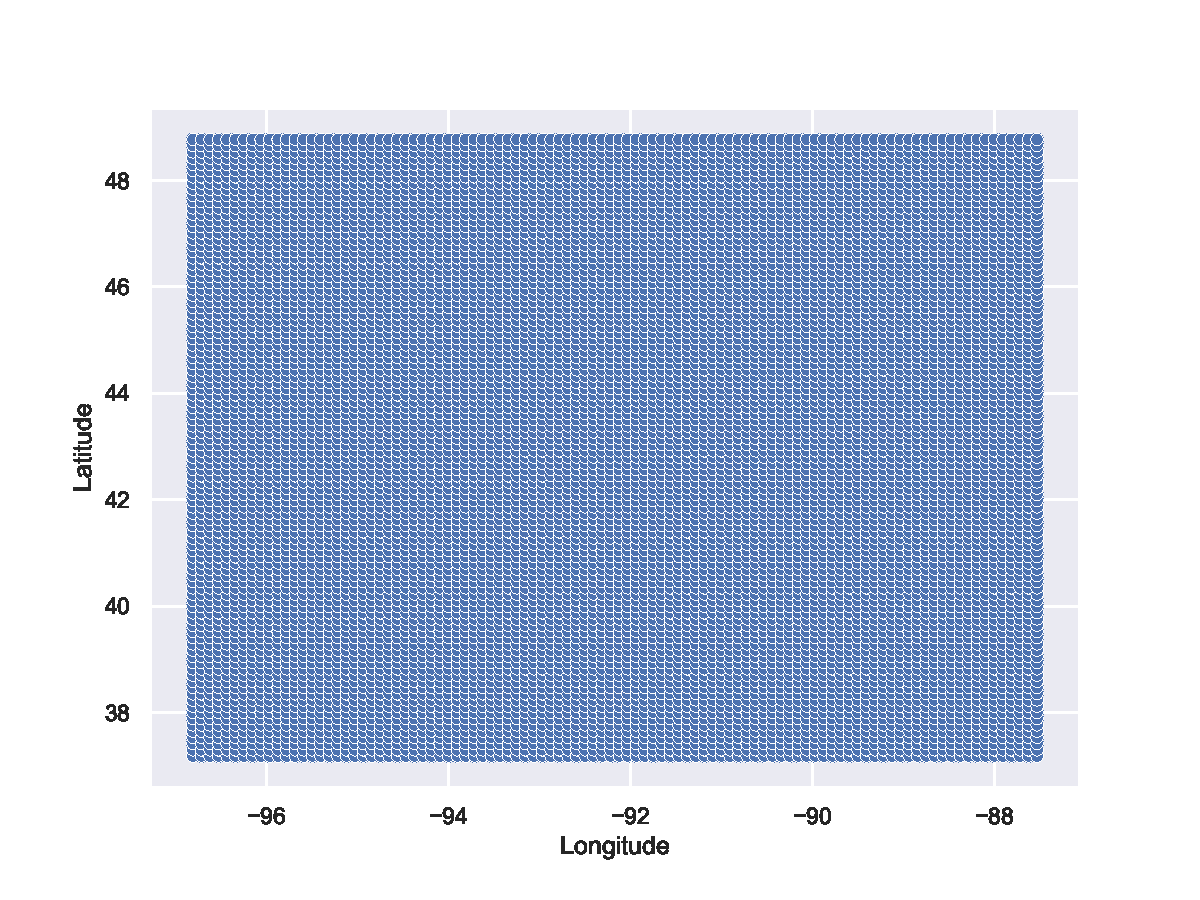
\includegraphics[width=\textwidth]{fig/Grid.pdf}
        \caption{Prediction Grid}
        \label{Prediction Grid}
    \end{minipage}\hfill
    \begin{minipage}{0.38\textwidth}
        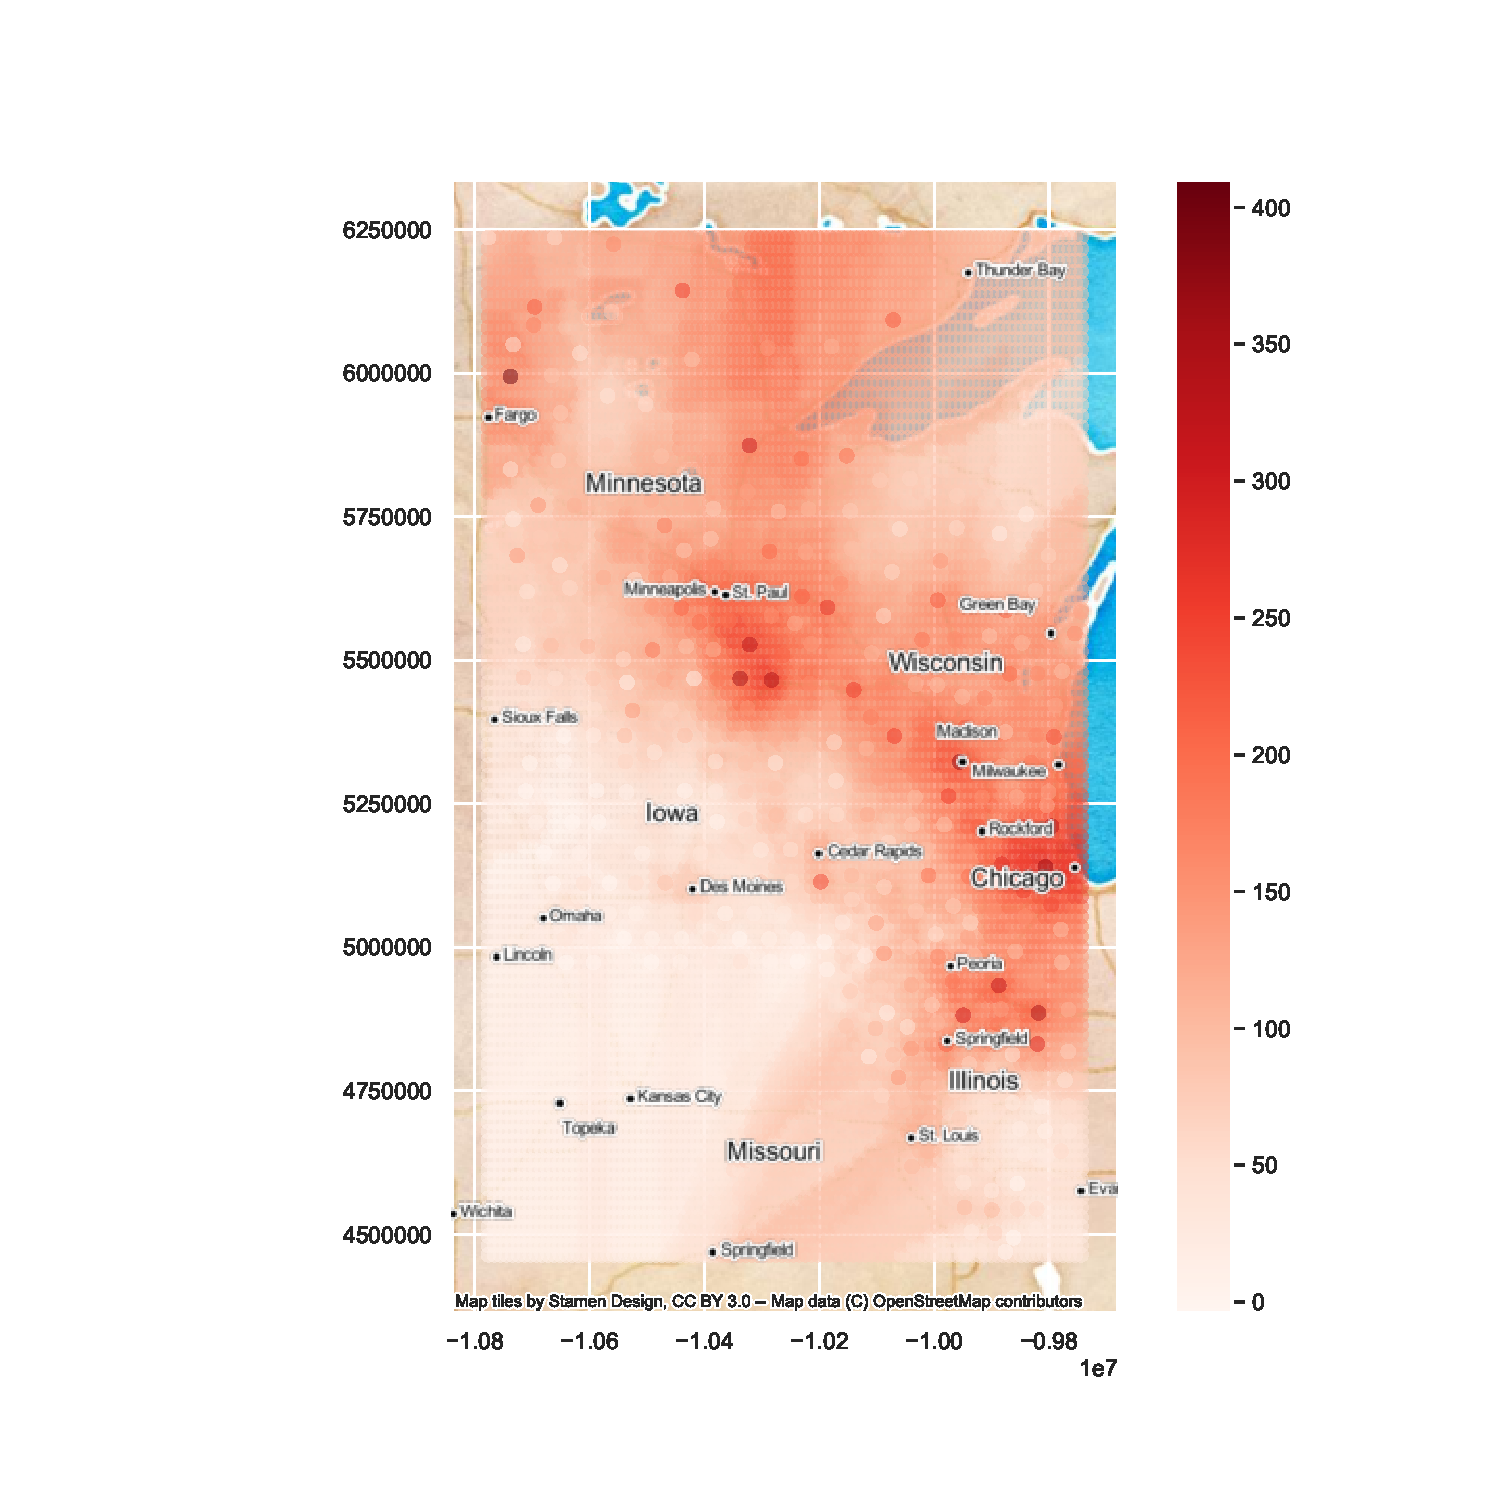
\includegraphics[width=\textwidth]{fig/Prediction.pdf}
        \caption{Prediction}
        \label{Prediction}
    \end{minipage}
\end{figure}




\section{Conclusion and Futurework}
% ∗ Summarize the biological answer to both questions; this summary should not include any numbers (2 points)
% ∗ Describe implications that these answers have for the larger biological context you described in the introduction (1 point)
In this report, we have modeled the spatial structure and the relationship between population and Covid-19 cases in Illinois, Iowa, Wisconsin and Minnesota. As a result, we found the spatial model is better than simple linear regression in terms of performance. The simple linear regression only reach a score of 0.1, and the spatial model reached a mean score of 0.48 with cross validation. The code is available at \href{https://github.com/Rexzhang99/Covid-19-Cases-Spatial-Prediction}{link}. 

From the result, we can see that there are indeed spatial dependence between the Covid-19 cases in different counties, and there is also a weak relationship between Covid-19 cases and population. 

However, there are still some limitations within our model. 
\begin{itemize}
    \item We did not using all data, we only considered Illinois, Iowa, Wisconsin and Minnesota.
    \item Due to time and data limitation we didn't consider other influential variables, such as age group, vaccination rate, 
    \item We should try more deterministic models with the regression kriging model, such as tree methods, support vector regression etc.
    \item When we acquire the geographic coordinates, some adrees  failed, we should find another way to get our data, such as Google Cloud Map API. 
    \item There are some out-liners in our data, when modeling the deterministic part, we should try some robust regression methods
\end{itemize}
In future-works, we should focus on the limitations of our model and trying to get a better result.  



% –References
% ∗ At least 5 references (2 points)
\bibliographystyle{plain}
\bibliography{ref}

\end{document}